\chapter{Performing in the air}\label{chap:touchless}

`Can you be my air guitar coach?' I still get calls from people that want to improve their air guitar skills, typically right before the annual Air Guitar Championships in Oulu, Finland. This is a fascinating competition in which people compete in mimicking the sound-producing actions of guitarists combined with extrovert communicative gestures. The reason people call me is that we researched air instrument performance \citep{godoy_playing_2006}. Our primary research focus was air piano, but we also did pilot studies on air drumming and air guitar performance. The latter was picked up by a journalist who named me `Dr. Air Guitar' in national media when I defended my dissertation in 2008. The fact is that I am no good at playing air guitar. However, I have over the years developed several \emph{air instruments} in which one can produce sound by moving in the air. This chapter looks at different types of air instruments and how they can be used in performance.


\section{Some considerations when designing air instruments}

Air instruments are built differently, but they have in common that the user controls sound by moving the body in the air. I will focus on three types of air instruments that I have explored over the years:

\begin{description}
	\item[Touchless air instruments:] This is the `purest' form of air performance, without holding anything in the hands. The Theremin is the classic example of such an instrument, played by moving the hands within the field of the instrument's two antennas.
  \item[Object-based air instruments:] Such performances are based on holding a motion-sensing device in the hands. Some devices have buttons and knobs, so they can also be used as traditional touch-based instruments.
  \item[Muscle-based air instruments:] These devices use the muscle tension of the performer to create sound. The most popular have been muscle-sensing armbands, but sensors can also be placed in other body parts.
\end{description}

Many of the air instruments we have developed at the University of Oslo have come out of our curiosity about how people move while listening to musical sound. This led to the experiments mentioned in Chapter~\ref{chap:motion}, such as the `air performance,' `free-dance,' and `sound-tracing' studies. The idea behind these studies was to understand more about people's music cognition by studying how they spontaneously move to musical stimuli. One finding from these studies is that air performance is ubiquitous. As would be expected, people with musical training are, in general, better at carrying out such tasks. For example, they are better at picking up on more layers in complex musical stimuli. We were more surprised by the capabilities of people with little or no musical training. Even people who claimed to be `tone deaf' or `unmusical' could follow various musical features in the air with one or more body parts. In essence, people are more musical than they believe.

If moving \emph{to} sound in the air is something everyone can do, what happens if we use this embodied music capacity to create new instruments? Several people have asked me to create an actual air guitar, a setup where you can play guitar-like sounds by moving in the air. There are already a couple of such examples \citep{karjalainen_virtual_2006,crawford_midi-airguitar_2009}, although both of those setups were based on (partly) handheld sensing. However, just like I do not find it particularly interesting to (re)create traditional acoustic instruments with digital technology, I am equally uninterested in creating `air versions' of traditional instruments. Instead, I am curious about new instrument concepts based on people moving in the air.

As briefly surveyed in Chapter~\ref{sec:motion-capture}, many technologies allow for capturing information about human body motion. It is impossible to say that one system works better than another; they all have positive and negative sides. The instruments I will present in this chapter are mainly based on two sensing types: inertial sensor-based units and infrared camera-based systems. The former is more flexible and embeddable. Inertial measurement units are small and can be placed anywhere on the body. This has made them popular in commercial products, which has helped lower the cost of such sensors. Camera-based systems are complex and costly in comparison. A multi-camera setup is less flexible to start with, and the setup is sensitive to light pollution and reflections. However, despite these drawbacks, camera-based systems can capture the exact location of an object in space with sub-millimeter accuracy and precision. So we have found such systems to be excellent for prototyping and some occasional performances. Knowledge from such exploration can later be implemented using other sensing technologies.

One of the challenges of working with motion tracking systems is the massive amounts of data they provide. A stream of full-body motion data typically contains up to 30 three-dimensional (sometimes six-dimensional) markers at rates above 100 Hz. It is impossible to map such data directly to a sound engine; multiple levels of data reduction and analysis techniques have to be applied. One approach is to identify `key postures' in the continuous motion stream based on a particular configuration of markers in time and space. If one uses a full-body motion capture system, this could be based on a kinematic model of the body. However, other constellations of markers or sensors could also work. Such posture recognition can be seen as a kind of `spatial thresholding,' looking at the spatial relationships between markers independent of time. This is an effective way to reduce the continuous stream of data since everything other than the identified postures will be discarded. One of the first examples of using camera-based motion tracking in real-time musical applications was a project by \citet{gang_qian_gesture-driven_2004} in which they used such static postures to drive the interactive system. This was done by dividing the body into ten `rigid objects' and using the object's angular relations as features in a pattern recognition system.

Posture-based tracking is a good starting point, but to utilize the potential of a continuous stream of motion data, one needs to find solutions for handling the temporal aspects of the stream. One approach is to perform some kind of action recognition based on `temporal segmentation.' Here the idea is to consider the temporal unfolding of motion. A straightforward approach is to calculate the running \emph{quantity of motion} (QoM). This is a `perceptual value,' meaning that it is calculated differently depending on the motion capture system in use. The point is to extract a feature that tells something about \emph{how much} motion there is at any point in time. This feature can then be used to segment the continuous motion stream into action segments based on a threshold. This way of thresholding the signal keeps more information than a purely posture-based analysis yet discards everything under the given threshold. Several of the first motion-capture-based instruments used this approach, such as in the music--dance performances created by \citet{dobrian_gestural_2003}.

Action-based tracking is challenging. A \emph{touchless action} can be defined as an action performed in the air without any haptic and tactile response. Everyone can do it, but it is challenging to figure out how to extract such an action from a continuous stream of motion data. One approach is to do something similar to how a MIDI-keyboard works. A keyboard passes on information about the finger's velocity during the key attack. The prefix and suffix of the action are irrelevant; the velocity of the attack is captured. One can do something similar by looking at the velocity of an object in space. The velocity will be zero when you switch direction while moving. Then one can use the energy profile leading up to the direction switch to control sound playback.  This is an example of relative action recognition. The action can be performed anywhere; it is the energy profile that defines the interaction. A different approach is to use an absolute spatial reference. Just as a physical instrument is located in one position, one could define an invisible `line' that one can `hit.' This is more in line with how a keyboard works.

Finally, a more high-level approach is to consider the meaning-bearing components of actions: the gestures. Many claims that they work with gesture-based interaction. However, according to my definitions, most such systems are motion or action-based. But there are some examples of systems that aim at extracting meaningful features from actions. For instance, Antonio Camurri and colleagues at the University of Genova have developed the EyesWeb computer vision software for extracting expressive features from video recordings \citep{camurri_tool_2005}. This software aims at capturing some of the \emph{quality} of the motion in question and using these data in the mapping process to musical features. One challenge, then, is that musicians are generally not trained at performing such expressive gestures. Most musicians spend time improving sound-producing actions on a physical instrument. When it comes to performing expressive gestures in the air, this is the domain of dancers. However, dancers often have little training in creating sounds. So gesture-based interaction is in a somewhat grey area between music and dance performance.


\section{Laserdance}\label{sec:laserdance}

My first exploration into `air performance' was in the music--dance project Laserdance. I met choreographer Mia Habib at the Norwegian centre for technology, art and music (Notam) in Oslo in 2001 and developed the sound interaction design for one of her pieces. In Laserdance, the scenography was based on a red laser beam splitting the stage floor (Figure~\ref{fig:laserdans02}), and the choreography explored this divided space. Passing the laser beam would trigger a sound, and the dancers explored moving in and out of the beam during the performance.

\begin{figure}[tbp]
		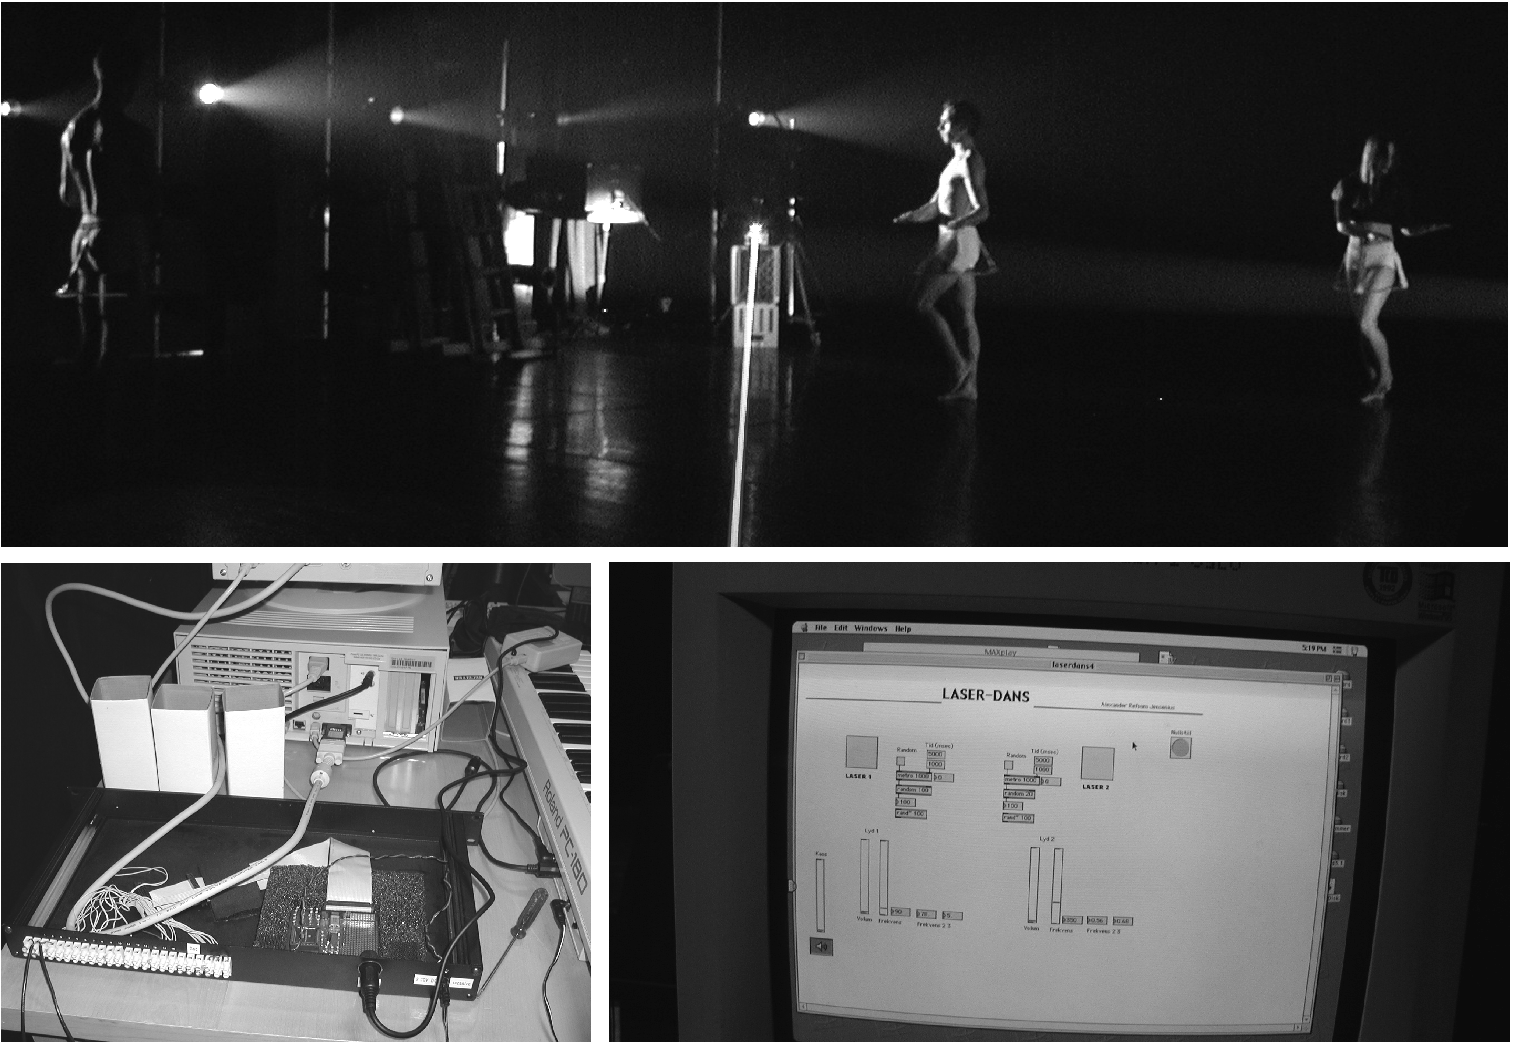
\includegraphics[width=\textwidth]{figures/70-laserdance-crop.pdf}
	\caption{The red laser beam split the stage in two during the performance of Laserdance (top). The technical setup was based on a custom-built Notam sensor interface and an infrared sensor (bottom left). The interactive sound design was implemented in Max/MSP (bottom right).}
	\label{fig:laserdans02}
\end{figure}

The technical setup was based around an infrared sensor pointed in the same direction as the laser beam and connected to a custom-built sensor interface. This interface sent out a MIDI control message whenever the dancer moved into the beam. The control message triggered playback of a synthetic sound based on frequency and amplitude modulation in a Max patch. As such, all parts of the action--sound mapping were quite basic: the control signal, the sound engine, and the mapping between action and sound.

Despite the simplicity of the design, the setup proved remarkably effective. This was at a time when most dancers had no prior experience with interactive music systems. So being able to control sound themselves on stage was an eye-opener. The dancers moved around on the dark stage and produced sound when `breaking' the laser beam. They did not control the sound beyond starting and stopping the playback, but that was enough to make a meaningful performance. The audience commented on the effectful combination of visuals and sound. The project showed that often simpler is better.


\section{Soniperforma}

Camera-based interactive systems often rely on the extraction of features from the video frames. For example, the quantity of motion of an object can be estimated by calculating the number of pixels that change between frames. This number can then be mapped to a sound feature. An entirely different approach is to \emph{sonify} the video, that is, create sound directly from the incoming data. This is the method used in the instrument Soniperforma \citep{jensenius_sonifying_2013}. Here I developed a technique I called \emph{sonomotiongram}, based on sonifying \emph{motiongrams}. A motiongram is a compact visual representation of motion images, made by `squeezing' together motion images to create a motion timeline \citep{jensenius_video_2013}. The sonomotiongram technique plays with the idea that motiongrams are visually similar to \emph{sonograms} (spectrograms of audio files). Sonograms and motiongrams are completely different visualization methods, but they may sometimes look alike. Therefore, I was curious about what would happen if I converted a motiongram to sound through an `inverse FFT' technique (Figure~\ref{fig:figures_time-frequency3}).

\begin{figure}[tbp]
	\centering
		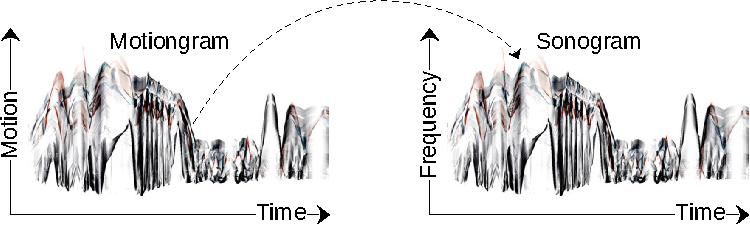
\includegraphics[width=1\columnwidth]{figures/71-sonomotiongram-crop.pdf}
	\caption{A sketch of the idea of sonifying motion through treating motiongram data as if it were a sonogram.}
	\label{fig:figures_time-frequency3}
\end{figure}

When converting an image into sound, one challenge is creating mappings between spatial (timeless) image features and non-spatial (temporal) audio features. In Soniperforma, data from the Y-axis of the motiongram is mapped to sound frequency. Data from the X-axis is used to control changes over time. Such a mapping from image to sound has been used several times in the past. An early example is the Pattern Playback machine built by a group of speech researchers in the late 1940s \citep{cooper_interconversion_1951}. This system made it possible to `draw' shapes that could be played back as sound. Iannis Xenakis' UPIC system from 1977 allowed for creating complex timbres by drawing with a digital pen on a computer screen \citep{marino_upic_1993}.  \citet{wenger_communities_1998} implemented similar ideas in the Metasynth software for sonifying images and photos.
These are examples of sonifying still images or moving images with a still character. There have also been experiments with sonifying moving images. For example, Norman McLaren created a series of short films in which he drew with a pen directly on the soundtrack of a 35~mm film strip \citep{jordan_norman_1953}. In the 1970s, Erkki Kurenniemi developed the video-based musical instrument Dimi-O to control sound synthesis from a video camera \citep{ojanen_design_2007}.

The sonification technique implemented in Soniperforma is conceptually similar to the examples mentioned above. One of the challenges is the `flat' spatial representation. When time is running along one axis, there is only one dimension to represent the spatial properties. A motiongram will only display motion in one spatial dimension: a horizontal motiongram visualizes vertical motion. Reducing three-dimensional motion into a one-dimensional display is a limitation. Still, preserving temporality helps represent the motion's `shape.' The result is an abstract yet connected auditory representation of the original motion.

As argued by \citet{winters_sonification_2012}, sonifying body motion is not the same as creating musically meaningful mappings. A sonification aims to convey information about the data, not to create an aesthetically exciting sound. At first, I mainly thought of the sonomotiongram technique as helpful in video analysis. By converting a video file to sound, I could quickly listen through hours of video recordings at high speeds to detect deviations in motion patterns that are difficult to see with the naked eye. As it turned out, I found that the technique was also a good starting point for music performance.

The software-based instrument Soniperforma was developed as a patcher in the graphical music programming language Max using a combination of Jamoma modules (Figure~\ref{fig:figures_soniperforma_soniperforma}). At the core of the instrument is the sonomotiongram algorithm, which converts the video stream to audio. As such, the mapping from motion to sound is fixed. However, I found that the sound could be controlled by modifying the incoming video. Changing the color, size, and orientation of the video image or applying visual effects would end up as sound effects. For example, a motion blur effect will end up as a sound delay. I have found this audiovisual interaction creatively inspiring as a performer. Since I often project my screen during performances, it is also an audiovisual experience for the audience.

\begin{figure}[tbp]
		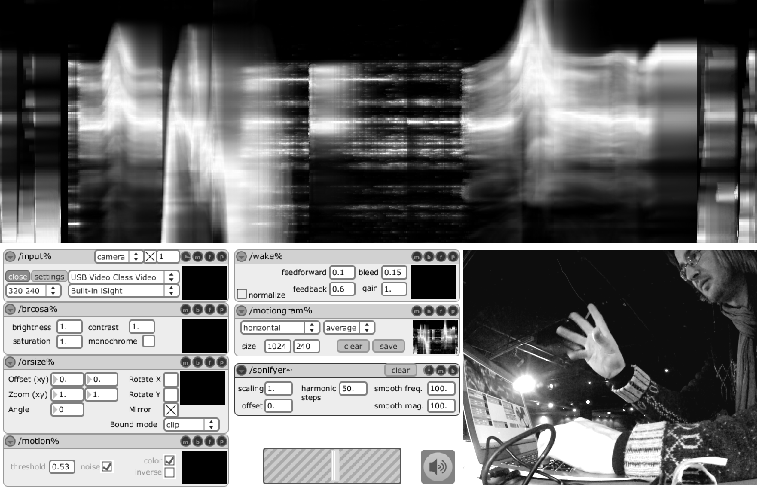
\includegraphics[width=1\textwidth]{figures/72-soniperforma-crop.pdf}
	\caption{The performance environment of Soniperforma, showing the Jamoma modules used for controlling the incoming video signal (bottom left), the motiongram used as the basis for the sonification algorithm (top), and the incoming video (bottom right).}
	\label{fig:figures_soniperforma_soniperforma}
\end{figure}

Its continuous one-dimensional interaction mode is both a strength and weakness in Soniperforma. For most physical instruments, it is possible to choose between sound-producing and non-sound-producing actions. For example, when playing the piano, only the keyboard actions produce sound. When playing with an instrument like Soniperforma, on the other hand, any motion in the image will show up in the motiongram and will be rendered as sound. Such a direct relationship between motion and sound is intuitive. One could even argue that it leads to a relatively small action--sound separation. Still, when performing with the instrument, I often wanted to turn the sound `on' and `off.' One solution to this `always-on' problem was to position the camera so that it could move out of the image. I also explored placing the camera at a 90-degree angle from where I stood. Then I could put my hands `into' the image when I wanted to produce sound similar to hitting a piano key. This effectively functioned as a manual action segmentation. The experimentation with Soniperforma sparked an interest in exploring how more advanced motion tracking could be used in interactive music systems.


\section{Kinectofon}

The ideas from Soniperforma were further developed when I got hold of a Microsoft Kinect `sensor.' They call it a sensor, but this device, initially developed for gaming, has two cameras: one regular video camera and one depth-sensitive camera. The latter captures the distance to the objects in the image. This device became the central part of a new prototype instrument, the Kinectofon \citep{jensenius_kinectofon_2013}. As shown in the signal flow in Figure~\ref{fig:figures_overview_overview}, Kinectofon uses the same sonomotiongram technique as Soniperforma. However, the Kinect allows for filtering the input image based on distance. This is done by combining the image from the depth-sensitive camera with a motion video from the regular camera. The result is a \emph{foreground motion image} based on the camera's desired distance.

\begin{figure}[tbp]
		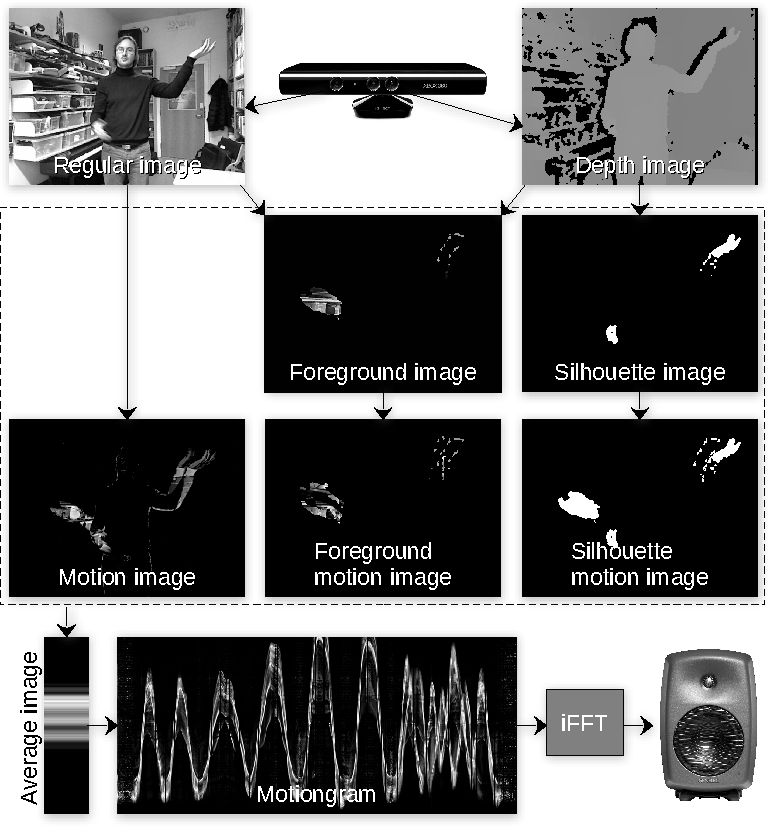
\includegraphics[width=\textwidth]{figures/73-kinectofon-crop.pdf}
	\caption{An overview of the Kinectofon signal flow. The two input images (regular and depth image) can be processed in various ways before they are passed to the average image module that creates the motiongram. Then the motiongram is converted to sound through the sonomotiongram technique.}
	\label{fig:figures_overview_overview}
\end{figure}

It is possible to create a foreground motion image with a regular video stream. However, that requires recording the background first to produce a reliable foreground image. It also helps to have a plain background, such as a single-colored wall. The advantage of a depth camera is that the `noisiness' of the background does not matter. It will effectively be filtered out when setting the depth threshold at the correct level. As I discovered, the depth functionality also allows for creating a performance `plane.' I can set the depth threshold half a meter in front of me when performing. Then I can stand in front of the camera and move my hands (and other body parts) `into' the image to create sound. This is an entirely different approach to performing in the air than with Soniperforma. `Touching' the plane almost feels like performing with a physical instrument. The invisible plane is fixed so you can touch the same spot and get the same sonic result. Many people that have tried the instrument have commented about this tactile illusion. The sonic interaction evokes mental imagery of physical touch.


\section{SoundSaber}

The air performance interfaces presented so far have all been touchless; the user performs with open hands in the air. An example of an object-based air instrument is the SoundSaber developed by my colleague Kristian Nymoen \citep{nymoen_soundsaber_2011}. This interface is built around a meter-long handheld rod that the performer moves in the air (Figure~\ref{fig:soundsaber}). The SoundSaber was initially developed to explore our new infrared motion capture system in the fourMs Lab at the University of Oslo. Later, it was developed into a barebone version using an accelerometer-based system. Common to both implementations was exploring how a seemingly simple sound synthesizer may come to life through high-quality sensing. Many commercial music technology products are opposite: `expensive' sound engines with poor control possibilities. SoundSaber exploits the high spatiotemporal resolution and low latency of the motion capture system, allowing for shortening the perceived action--sound separation.

\begin{figure}[tbp]
	\centering
		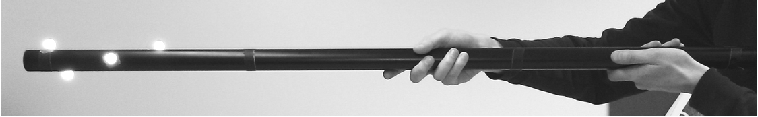
\includegraphics[width=\columnwidth]{figures/74-soundsaber-crop.pdf}
	\caption{The SoundSaber rod has reflective markers attached in a specific constellation so that it is possible to track both its position and orientation (Photo: Ståle A. Skogstad).}
	\label{fig:soundsaber}
\end{figure}

The mappings in SoundSaber were inspired by the many-to-many mappings found in acoustic instruments. One could imagine that tracking only one point in space---the tip of the rod---would lead to a somewhat limited interaction. However, SoundSaber has a clever solution to retrieve as much information as possible from the motion capture data. Attaching multiple markers on the rod makes it possible to define a `rigid object' that can be tracked with both three-dimensional position (X, Y, Z) and three-dimensional rotation (pitch, yaw, roll). This six-dimensional data stream can be used to calculate the absolute and relative velocity and acceleration in both polar and cartesian coordinates.

The SoundSaber's sound engine is based on a sequence of short clicks sent through a chain of delay lines, a ring modulator, another delay line, and a bandpass filter. The first action--sound mapping, mimics the `energy transfer' of a sound-producing action by controlling the sound's amplitude with the absolute velocity of the rod. The rod's absolute horizontal position is used to control the sound's spatial location, utilizing the multi-channel speaker system in the lab. Thus the user can `move' the sound around in the space. The absolute vertical position is used to control pitch information, with lower frequencies closer to the floor. The combination of absolute and relative mappings means that the user can produce similar sounds independent of the direction faced, similar to what one would expect from a handheld acoustic instrument.

Everyone that has tried SoundSaber comments on its highly expressive nature. I think there are three reasons why it works so well. The first is the high spatiotemporal resolution. We usually run the motion tracking at 200~Hz and with millimeter-level precision. This makes for both immediate and intimate interaction. The mappings are made so that both large and small actions affect the sound. Most users move the rod with large actions, but even rapid finger tapping will produce some audible sound. This creates the feeling of playing an instrument with a large dynamic span, both in action and sound. Another reason SoundSaber works well is its many-to-many mappings. This mimics the complex mapping found in many acoustic instruments. Finally, the rod provides users with the tactile feel of holding onto a metal surface. Its size, shape, and mass give users a haptic experience based on the inertia when moving it around.

The most significant limitation of SoundSaber is that it is bound to our lab. In theory, the setup can be moved elsewhere or be set up in a similar lab elsewhere. However, to test the concept in a more portable format, we recreated the instrument using a Nintendo Wiimote. This controller is based on inertial sensing and cannot track position directly. However, the orientation can be estimated quite precisely, and the accelerometer data can be used to calculate the `energy' used in the instrument. It turned out that only some of the original SoundSaber mappings could be `ported' to the new setup. For example, even though we could extract the angle between the floor and the controller, the orientation data turned out too noisy to be helpful. It was also tricky to recreate the energy transfer function reliably. We, therefore, had to revert to using one of the pushbuttons on the Wiimote to turn the sound on and off. The reimplemented SoundSaber is fun to play, but it deviates substantially from the original. The fact that it relies on a trigger button also means that it is no longer a `true' air instrument.


\section{Dance Jockey}

Dance Jockey is an instrument based on full-body motion tracking using an inertial sensor system (Figure~\ref{fig:Mostra}). It is in many ways the complete opposite of SoundSaber. While SoundSaber is based on multi-layered continuous mapping from motion to sound, Dance Jockey uses mappings based on posture recognition. Dance Jockey was developed at the University of Oslo by Yago de Quay and Ståle Skogstad with the aim of catering for interactive dance performances \citep{skogstad_osc_2011,de_quay_dance_2011}. It was from the onset targeted at performances in real-world venues, so we decided to use a commercially available portable inertial motion capture suit (Xsens MVN Biomech). The suit has 17 inertial sensors attached to the body. Each sensor consists of a 3D accelerometer, a gyroscope, and a magnetometer. These are used to calculate both the three-dimensional position and rotation of a total of 22 body joints. This means that the data stream consists of 132 data points coming in at 120 frames per second. The challenge was to figure out how to meaningfully map this high-dimensional data set to sound and music features.

\begin{figure}[tbp]
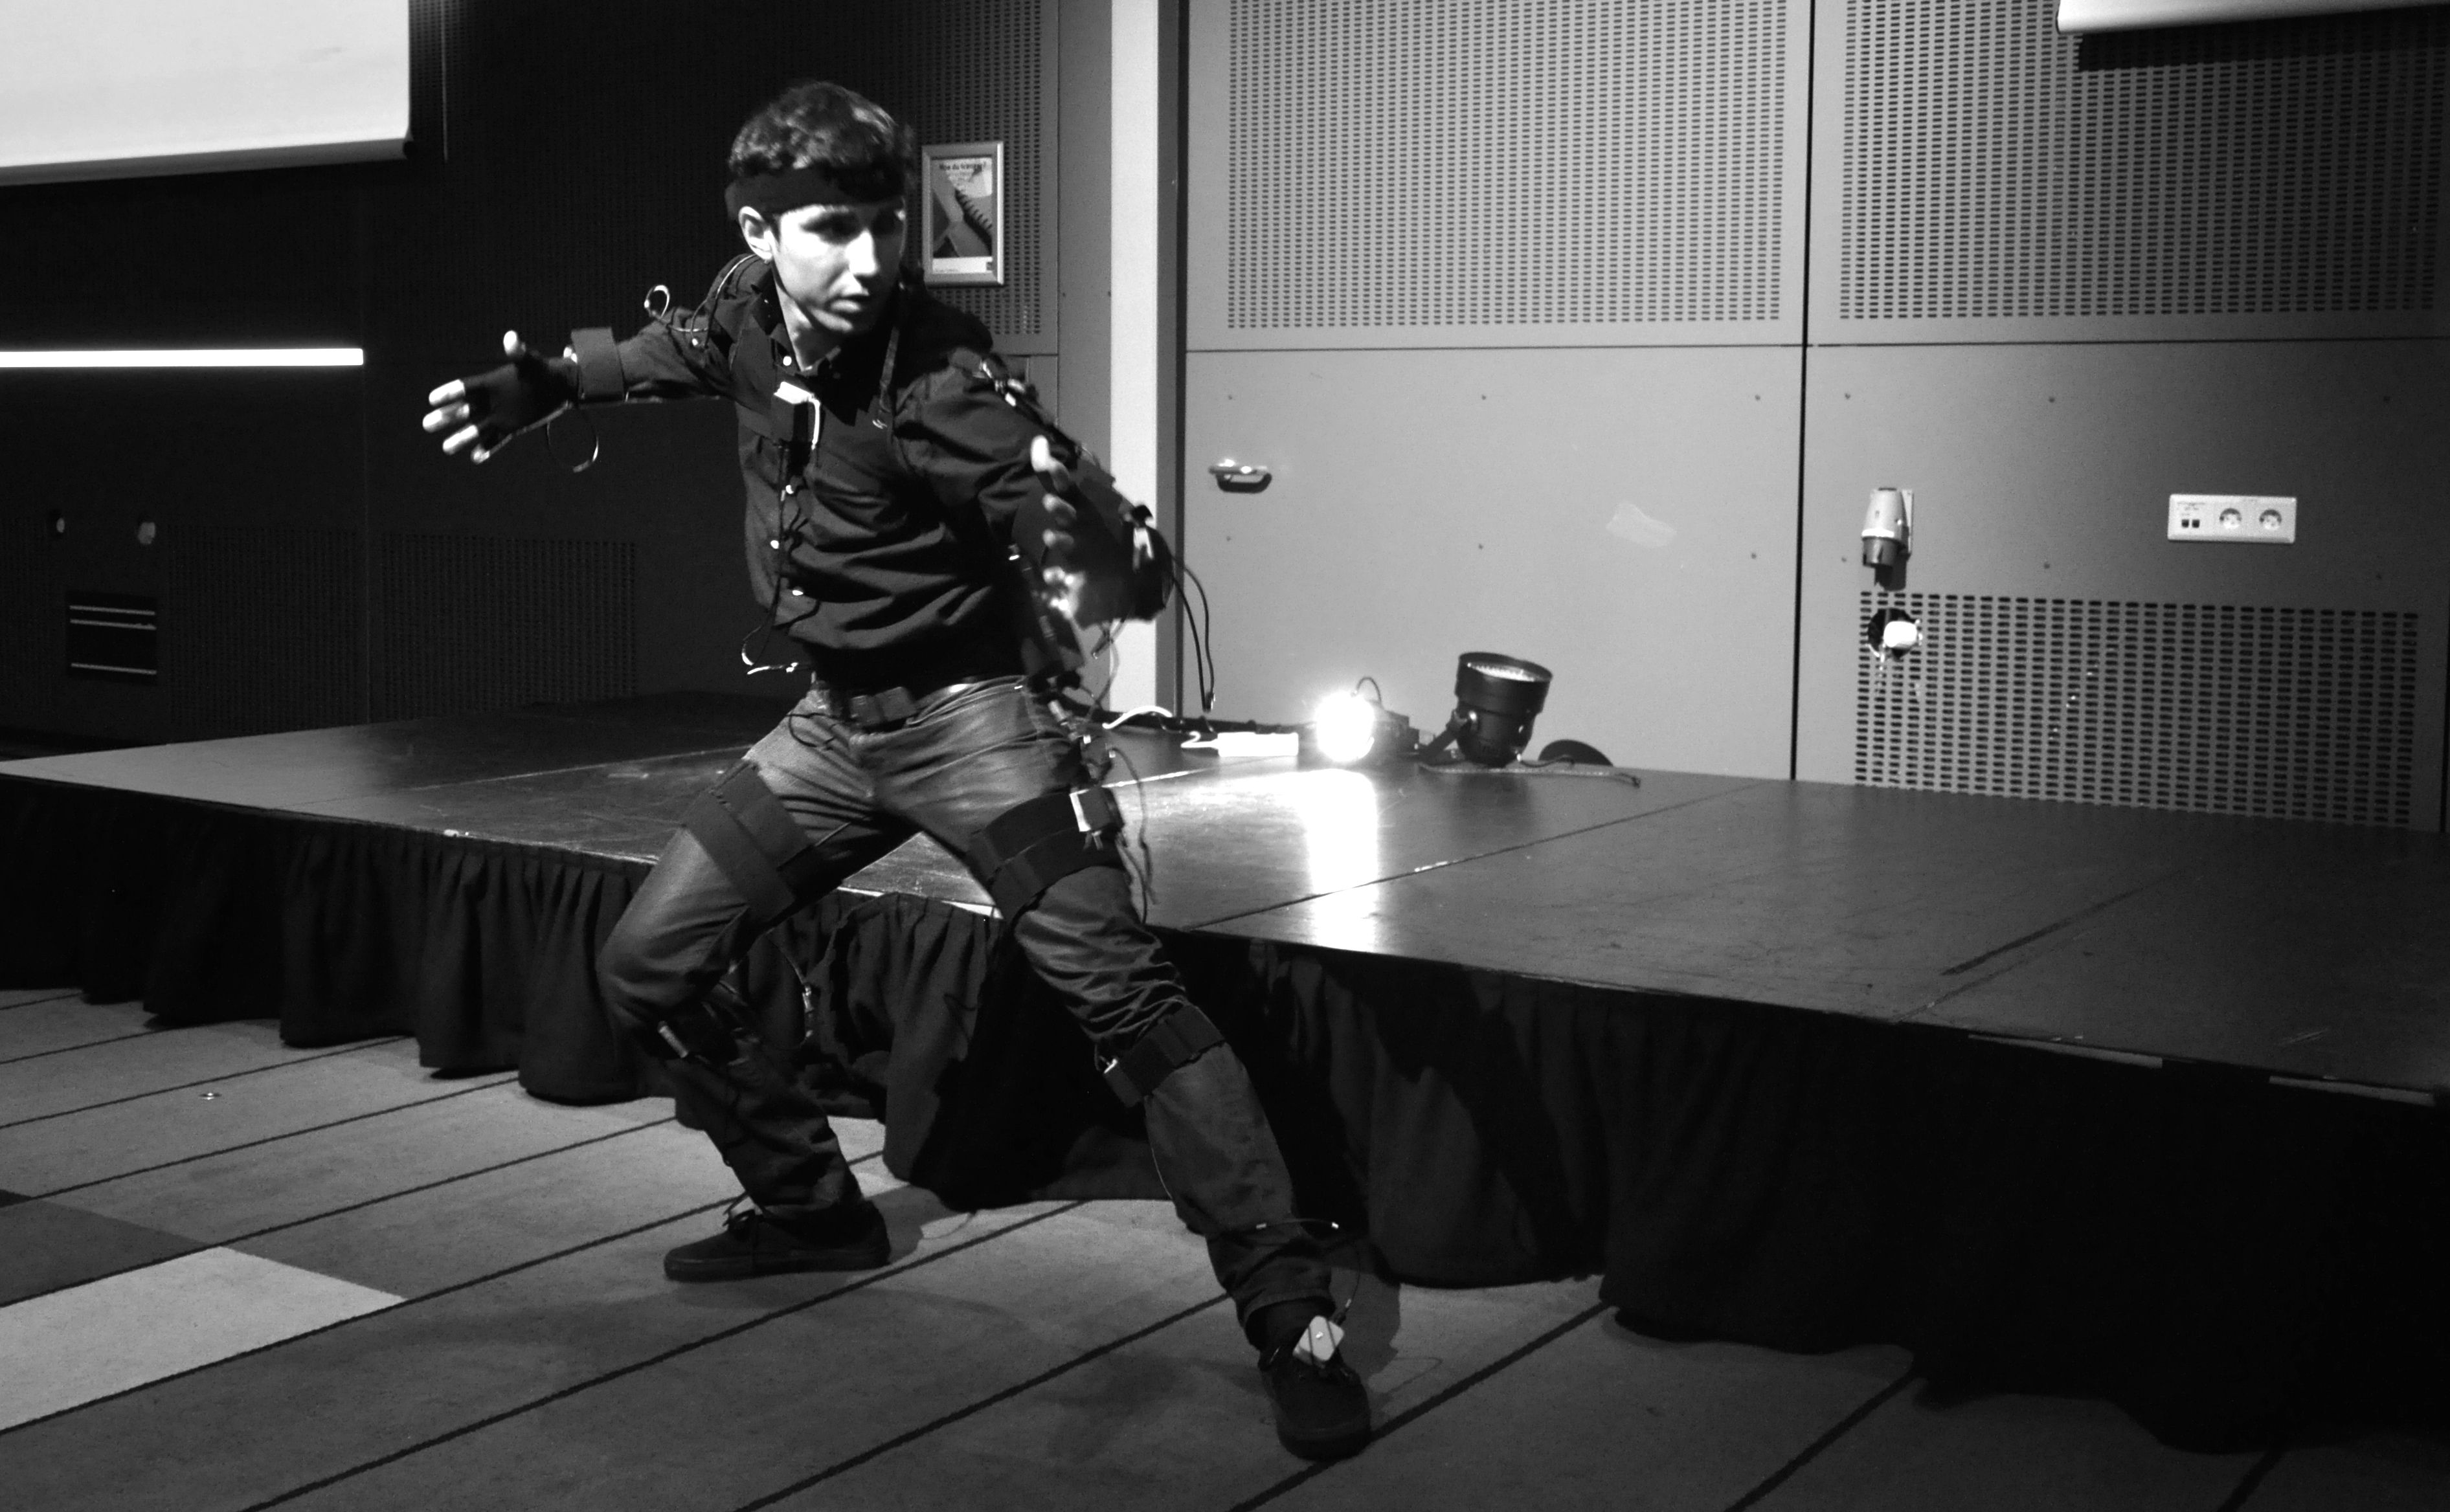
\includegraphics[width=1\columnwidth]{figures/75-dancejockey.jpg}
\caption{A Dance Jockey performance by Yago de Quay in Oslo, November 2010. The performer wears the Xsens MVN motion tracking suit containing 17 inertial measurement units connected to a wireless transmitter.}
\label{fig:Mostra}
\end{figure}

As the name suggests, Dance Jockey was inspired by a `disk jockey' approach to musicking. Instead of creating new sounds from scratch, the performer would trigger samples and add sound effects. This was achieved through a combination of continuous and discrete controls. Since the Xsens suit uses inertial tracking, we decided early on to work with relative position information. That means looking at how much and in which direction motion happens rather than its exact location in space. The system can provide absolute position information, but we experienced a considerable positional drift in our laboratory tests \citep{skogstad_osc_2011}. To ensure stable operation, we instead decided to work with relative motion information.

A benefit of working with full-body motion tracking is that one can calculate relationships between different body joints. In Dance Jockey, we extracted three relative position features describing body limbs and their relationships: the hand distance, elbow angle, and the body's level of contraction or expansion. The latter was implemented as the distance between five body extremities: head, hands, and feet. We also implemented `trigger areas' in the space around the user. These were used to play on virtual `wind chimes' that could be reached by stretching the arms and `touching' the relevant areas around the standing position. The primary shifts in performances were triggered by a hand `clap' feature. The performer could start a new part of the performance by moving his hands closer than 20 cm from each other. This and other static features were calculated using a `posture classifier' based on the angles between different body joints. These angles are relative to the performer's body and are easily reproducible once appropriately trained. Finally, hand speed was used to control the sound level, creating a relationship between the quantity of motion and sound level.

We found that a well-trained posture recognition system is more reliable than action recognition. Discarding temporal information and focusing only on spatial relationships between body parts efficiently reduces the data stream. However, the downside to working with posture recognition systems is that they favor trigger-based mappings. This works well for systems based on sample playback, but it does not allow for continuous control. To draw an analogy to acoustic instruments, one could say that a posture-based instrument is like a piano, while an action-based instrument is like a violin.

The Dance Jockey system was successfully used in several performances. Most performances were based on using an external PA system for the sound playback. We also experimented with the performer carrying the processing computer in a backpack and holding mobile speakers in his hands. Unlike the previously mentioned air instruments, Dance Jockey was more of a music-maker than a sound-maker. Entire compositions were programmed into the instrument. This made for engaging musical experiences, but the system could not be used for anything else.


\section{Sverm micromotion instruments}\label{sec:sverm}

After researching music-related body motion for a decade, I realized that all my studies and instruments were based on relatively large-scale body motion. I, therefore, decided to shift attention and delve into the world of human \emph{micromotion}. This was after I met dancer--choreographer Kari Anne Vadstensvik Bjerkestrand, a tai chi practitioner and slow-motion enthusiast. Together, we began a practice of standing still together. We ran sessions where we stood still on the floor for 10 minutes at a time in the motion capture lab. We measured our swaying and carefully wrote down notes about the sessions to compare the qualitative and quantitative data. As can be imagined, it is impossible to stand absolutely still. And when one attempts to stand still for a while, the body's micromotion comes to one's attention. This artistic exploration later turned into a scientific research project in which we have found that people's head sway at an average rate of up to around 10 mm/s \citep{jensenius_musical_2017,gonzalez_sanchez_correspondences_2018,gonzalez_sanchez_analysis_2019,zelechowska_headphones_2020}. The exact quantity of motion is not the most important; the main point is that micromotion is significantly smaller than what is normally considered in interactive music systems.

The initial standstill study developed into the artistic research project \emph{Sverm}  in which we worked with the micromotion and microsound found when approaching standstill. Here we developed a \emph{spatiotemporal matrix} as a tool for guiding us in rehearsal \citep{lesaffre_sonic_2017}. This matrix consists of three spatial and three temporal levels: micro, meso, and macro. Normal actions can be considered as the `meso-meso' level: in the range of approximately 1--100~centimeters and 0.5--10~seconds. It is possible to think of a `micro--micro action' as an action in micro-space (less than 1~centimer) and micro-time (shorter than 0.5~milliseconds). Anything above 100~centimers and 10~seconds would be considered a `macro--macro action.' In rehearsals, we tried to perform combinations of micro, meso, and macro actions. For example, we could perform a series of micro--micro actions in 10-second intervals for 5 minutes. Then we could switch to performing a micro--macro action over ten minutes. As can be imagined, these extreme cases were the most difficult to master, but they were also the most interesting to work with \citep{jensenius_exploring_2012}.

After training up our sensitivity to performing with microactions over several months, we developed what would become a series of instrumental concepts based on what I have called \emph{sonic microinteraction} \citep{lesaffre_sonic_2017}. One could argue that many acoustic instruments are built around microinteraction, such as the minute actions found in wind performers' mouths or the fingering of string players. Some electro-acoustic instruments also exploit such detailed control of sound, such as the multidimensional controllers presented in Chapter~\ref{sec:mpe-instruments}. However, there are few examples of air performance instruments exploiting microinteraction. The limitation is not on the sensing side. Nowadays, both inertial and optical motion capture systems are capable of detecting micromotion, something we have documented in various technology experiments  \citep{skogstad_comparing_2011,jensenius_study_2012,nymoen_comparing_2012,bishop_reliability_2020}. In my experience, the limitations are mainly on the conceptual side.

Waving Sines was my first microinteraction instrument \citep{lesaffre_sonic_2017}. It was conceived after some initial tests of sonification of the continuous motion data stream from the motion tracking system. I decided to map the vertical position of a motion capture marker directly to the frequency of a sine tone generator. This is probably the simplest motion--sound mapping, yet it turned out to be remarkably interesting. Sine tones are usually perceived as static, but when controlled by a high-speed motion tracking system, the sound came `alive.' I continued the testing by mapping the quantity of motion to the sound level. This made it possible to make sound only when moving. At some point, I did something wrong in the programming and ended up with a reverse mapping; sound would only appear when there was no motion. If one moved, there would be no sound. This is counter-intuitive, yet we all felt that it was inspiring to work with. In Waving Sines, we utilized this `inverse control' paradigm in performance (Figure~\ref{fig:trial}). The performers each wore a reflective marker on their heads. Since the marker's vertical position was mapped to the frequency of a sine tone, a taller person would produce a higher pitch than a lower one. The horizontal position controlled the spatial location of sound when played back over a multi-channel sound system. The twist is that sound is generated by standing still; motion leads to silence.

\begin{figure}[tbp]
	\centering
		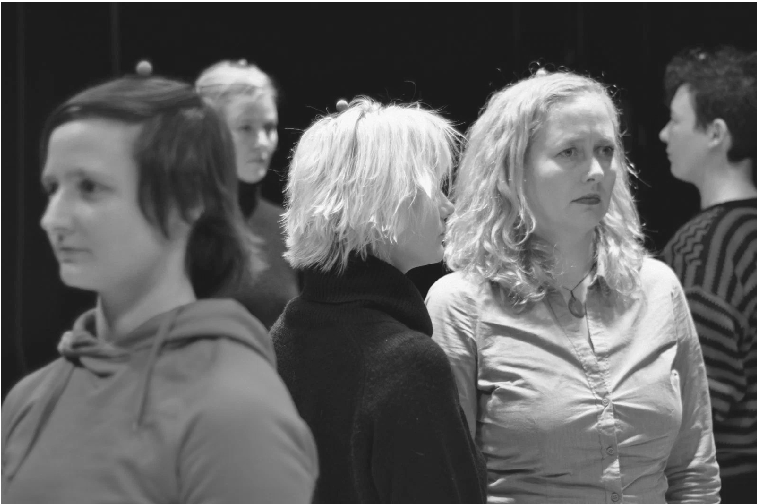
\includegraphics[width=1\columnwidth]{figures/76-waving-sines-crop.pdf}
	\caption{Rehearsing with the Waving Sines instrument for one of the performances of the \emph{Sverm}  project. Each performer inversely controls a sine tone based on the tracked position of a reflective marker on the head.}
	\label{fig:trial}
\end{figure}

Performing with an instrument built around inverse sonic microinteraction is more complicated than it sounds. Such a mapping is counter-intuitive by design. That is also what makes it fascinating. Once you master producing sound by standing still, you want to try modifying the pitch. However, this requires moving (a little). However, as soon as you move, the sound disappears. As we rehearsed with the instrument, the performers chose different strategies. Some just gave up on controlling it continuously and decided to play by standing still for a while, then move to a new posture to get another pitch. Others managed to move very slowly while maintaining a continuous sound. This works if your motion is small and slow enough. However, due to the high accuracy and precision of the motion capture system, such micromotion will lead to small fluctuations in both amplitude and frequency of the sound. That is what makes the sonic result of the instrument interesting. Listening to a static sine tone can be annoying. However, listening to multiple sine tones that continuously change in both amplitude and frequency makes the sound come alive. The sounds are shaped by the swaying and breathing of the performers.

Waving Sines can be performed alone, but it was developed as a collaborative instrument. I particularly enjoy listening to how the different sine tones blend when multiple perform. If you have people of the same height---or if they adjust their heads to the same vertical position---one may get \emph{beat} frequencies. That is, one may hear a pulsation based on the difference between the individual frequencies. Once, I had a group of students who spent a good half hour aligning themselves to create such complex beat patterns. Another group explored playing harmonies together by positioning their heads accordingly. Of course, all such explorations are made more challenging because sound disappears once you move.


\section{Muscle performance}\label{sec:muscles}

Waving Sines and the other microinteraction-based instruments we developed in the \emph{Sverm} project were all based on camera-based motion tracking. To move outside of the lab, I got curious about testing other sensor types and sensing modalities. Then muscle sensing quickly comes to mind. Muscle activity can be measured using \emph{electromyography} (EMG), one of the most commonly used biosignals for musical applications \citep{aly_appropriating_2021}. \citet{knapp_bioelectric_1990} did pioneering work on EMG-controlled music in the 1990s. His BioMuse system has been used by several others, of which the work of \citep{tanaka_musical_1993} is perhaps the most well known. There are also examples of using muscular \emph{sound} in performance, such as in the works by \citet{donnarumma_configuring_2016}. His Xth Sense system can be seen as a hybrid electro-acoustic instrument since it amplifies and modifies acoustic sound generated in the body.

Specialized muscle sensing equipment has been available for decades. Still, it was the advent of the commercially available Myo armband controller in 2014 that sparked a broader interest in using muscular control in interactive music systems. Not only is the Myo armband easy to use with its eight muscle sensors, accelerometers, wireless connection, and rechargeable battery, but the data is also of sufficiently high quality to be used for musical applications \citep{nymoen_mumyo_2015}. We also verified that it could sense micro-level activity \citep{jensenius_Exploring_2017a}. Unfortunately, the armbands went out of production after some years, but we still have a collection of devices that we continue to explore at the University of Oslo.

One of the instruments we have built around a Myo armband is the MicroMyo instrument. This is a complete instrument containing a small Bela-based microcomputer \citep{mcpherson_environment_2015}, a battery pack, and a portable speaker \citep{martin_composing_2018}. This portable design makes it easy to perform in any location. In the piece \emph{Stillness Under Tension} we explored the MicroMyo instrument in a collaborative performance setting (Figure~\ref{fig:performance}). Here the mappings were based on the same inverse control principle as Waving Sines. The performers need to stand still for sound to appear. When the performer moves, the sound fades out quickly.

\begin{figure}[tp]
\centering
\includegraphics[width=\columnwidth]{figures/77-micromyo.jpg}
\label{fig:sverm-myo-performance}
\caption{The premiere of \emph{Stillness Under Tension} in Oslo in November 2017. Each performer wears a Myo armband on their hand, capturing motion, rotation, and muscle tension in the arm (Photo: Simen Kjellin).
}\label{fig:performance}
\end{figure}

The Myo armband provides relative motion information through the inertial sensor. Here we found the data from the embedded gyroscope to be most reliable. So we could use arm rotation to control the base frequency of the sound engine. Holding the arm down will result in a lower pitch. Data from the eight muscle sensors were mapped to frequencies of individual partials in an additive synthesizer. This made it possible for each performer to control the sound's timbre by flexing their arm muscles. They had to do this carefully since the sound would fade out if they moved too much. Similar to Waving Sines, the performers had a constant `battle' between trying to move and not move at the same time.

Even though MicroMyo and Waving Sines are based on the same conceptual idea, their implementation is entirely different. In Waving Sines, the performers wear a single, lightweight marker on top of the head. This encourages standing upright and focusing on swaying back and forth or moving slowly up and down. The sensor armbands used in MicroMyo focus the attention of both performers and perceivers on the arm. Thus the two instruments afford completely different musical interactions.

Waving Sines is based on a multi-camera motion capture system, a multi-channel sound system, and two PCs. In theory, it is possible to move the setup. In practice, it is only used in our lab. MicroMyo, on the other hand, is a portable instrument. The complete instrument can fit in a small bag, including the handheld speaker. The result is that I regularly both demonstrate and perform with MicroMyo in various settings, while I only occasionally start up Waving Sines for a demonstration in the lab. The ideas from MicroMyo have also developed into other similar setups, such as in the music--dance piece Vrengt \citep{erdem_towards_2020}.

I want to dwell on the fact that MicroMyo is running on an embedded system. The prototype of the instrument was developed on a laptop \citep{jensenius_Exploring_2017a}. This worked, but we found it unreliable in performance, primarily because of Bluetooth connectivity problems. The setup did not scale well either since one laptop was needed per armband. A six-person performance required a quite large technical rig, with the added complexity of simultaneously getting six computers up and running. There was always some issue: a software update notification, the failure to load a package, or a Bluetooth connectivity problem. These are common challenges for computer-based setups and are usually easy to solve. Still, I find such issues problematic in performance contexts with limited setup time and where the systems need to be left alone for some time between setup and performance.
Then working with embedded systems is much more comfortable. After reimplementing MicroMyo using small Bela computers \citep{martin_composing_2018}, the whole setup consisted only of the armband, the microcomputer, a battery, and a speaker. This meant that each performer could carry their instrument and be in complete control of its operation. The importance of using single-purpose microcomputers in musical instruments should not be underestimated \citep{berdahl_satellite_2011}. Having an embedded system has made the instrument more user-friendly. One just puts on the armband, turns on the microcomputer and speaker's power, and starts producing sound.

My excitement for embedded systems coincides with a general interest in more `hardware'-based devices. I am writing `hardware' here because while MicroMyo and other similar instruments may be considered standalone devices, they contain a computer. The main difference is that it is a dedicated and stripped-down computer that is only supposed to do one thing. It is interesting to witness the `cyclic' nature of technological development. At the beginning of the digital era, all systems were single-purpose devices. As more powerful computers appeared, people would interact with these servers through `thin' clients. These thin clients were overthrown by the personal computers in the 1980s, laptops at the turn of the millennium, and tablets and mobile phones from the 2010s. Today, we see an increased interest in server-based solutions and embedded systems again. One reason for this is that larger and more powerful does not necessarily mean faster. \citet{mcpherson_action-sound_2016} have shown that an embedded platform can have a lower action--sound latency than a laptop-based system. Making complete standalone instruments most likely also ensures a longer lifetime for those instruments.


\section{Self-playing guitars}\label{self-playing-guitars}

The last series of air instruments I will present in this chapter is based on a concept we call the \emph{Self-playing guitars}. We have developed this platform over the last few years at the University of Oslo, resulting in several different installations and performances. The first of these, the installation \emph{Sverm--Resonans} consisted of six actively augmented acoustic guitars (Figure~\ref{fig:sverm-resonans}). Each of these could be considered a self-contained electro-acoustic instrument, and the whole installation could probably best be described as a large meta-instrument.

\begin{figure}[tp]
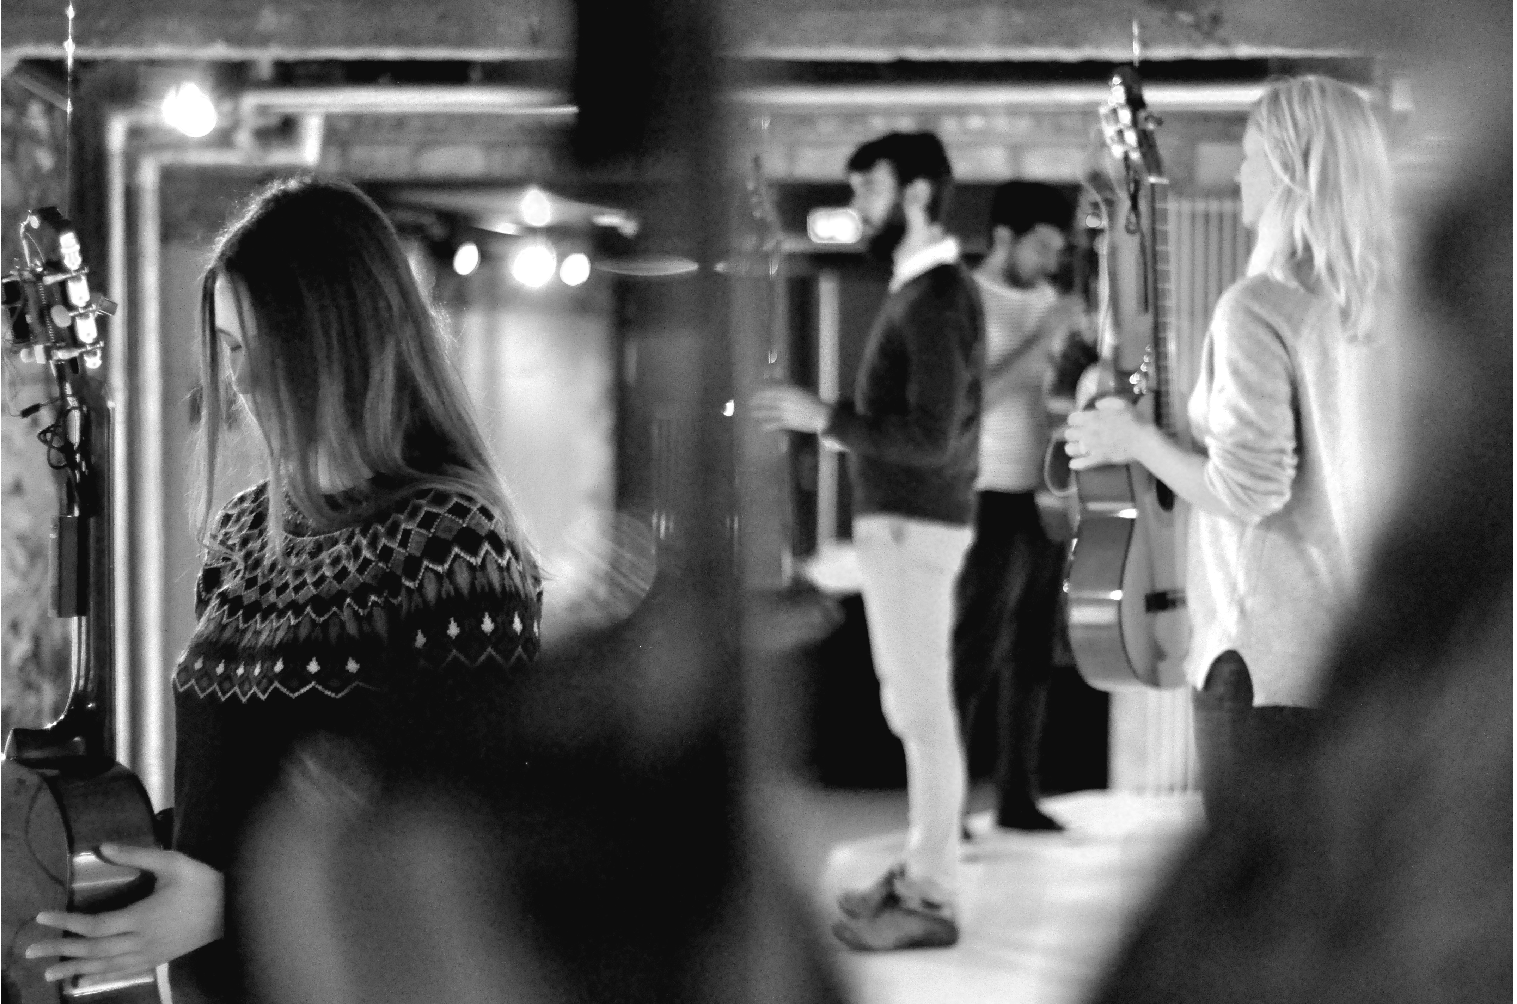
\includegraphics[width=1\columnwidth]{figures/78-guitars-crop.pdf}
\caption{A performance with the installation \emph{Sverm--Resonans}. Each guitar is an independent instrument controlled by the microinteractions of a still-standing human.}
\label{fig:sverm-resonans}
\end{figure}

The Self-playing guitars are not really `touchless.' In fact, we often encourage touching and holding them. However, the \emph{control} of the guitars is touchless, and conceptually they have been developed based on the ideas of standstill and inverse microinteraction that came out of the \emph{Sverm} project. The main difference between the Self-playing guitars and the other instruments I have described earlier in this chapter is the focus on the electro-\emph{acoustic} sound played through the body of the guitars.
There has been a growing interest in the augmentation of acoustic instruments in recent years, ranging from augmentations aimed at helping people to learn an instrument \citep{heller_augmented_2017,baldwin_tromba_2016} to tools for expert performers \citep{reboursiere_multimodal_2010,kimura_extracting_2012,lahdeoja_augmented_2015}. One reason for this trend may be to exploit the richness and non-linearities of acoustic sound generation while simultaneously utilizing the power of digital sensing and control.

The artistic goal of the installation \emph{Sverm--Resonans} was to invite people to connect with their breathing and give them time and space to relax. This was something we had seen that people responded positively to in the \emph{Sverm} performances. Now we wanted to see if we could generate some of the same effects in a gallery space. The installation was conceived as a meeting point between a living body interacting with an electronic sound system played through a vibrating acoustic instrument. As such, \emph{Sverm--Resonans} explored the meeting points between the tactile and the kinesthetic, the body and the mind, and between motion and sound. Each guitar produced a quiet low-frequency drone while hanging. This created a sonic ambiance in the gallery space. They were mounted in thin fish lines, which made them rotate slowly. The result was a stable yet continuous sound in the space.

The interaction with the guitars was based on the same inverse control idea explored in some of the previous instruments. The guitars had an infrared sensor attached to the neck, which would detect a person standing in front. After a few seconds of standstill, the guitars would gradually produce sound. This was a slow breathing-like sound aimed at helping people to focus on their respiration cycle. The pitch of the breathing sound would slightly change based on a person's distance to the guitar. If moving beyond a specified threshold, the breathing-like sound would disappear. Then one had to stand still again and wait for the sound to reappear. Working on the prototype, we discovered the tactile and haptic experience of holding the vibrating guitars. For the installation, we, therefore, encouraged people to hold the guitars. Many did, but the interaction also worked if someone just stood still without holding.

Each of the guitars is an independent and self-contained instrument, equipped with a microcomputer, various sensors, an actuator, and a battery pack \citep{gonzalez_sanchez_bela-based_2018}. There are no external speakers; all sound is generated by the actuators mounted on the back of the guitars. On the sensor side, one infrared distance sensor measures the proximity of people, an inertial measurement unit picks up motion and rotation, and a microphone `listens' to sounds in the space. Together, this provides a flexible and powerful electro-acoustic instrument. The guitars can easily be reprogrammed using various music programming languages (PureData, Csound, SuperCollider). One thing that has become clear is the need to fine-tune the sound engines to the instrument. Standard speakers have a relatively flat sonic response, while the guitars have a strong sonic identity. Therefore, it is essential to develop sound engines and create mappings between sensors and the sound features that match the guitars' sonic characteristics. This has been a useful reminder about the importance of considering the whole chain from action to sound when designing instruments.

Over the years, we have explored many different sound designs with the guitars. The \emph{Sverm--Resonans} installation was meditative. In \emph{Sverm--Puls} we explored a rhythmic sound design based on \emph{entrainment} principles. Entrainment is the process with which individual rhythmic patterns interact with each other \citep{clayton_interpersonal_2020}. Our entrainment implementation was based on the firefly-inspired design suggested by \citet{nymoen_decentralized_2014}. When left alone, the guitars entrain to a common pulse based on time-shifting their pulsations to a common pulse. This is done by `listening' to the environment using built-in microphones. The idea is that other sounds `distract' the entrainment process, thereby creating a more complex soundscape. The infrared sensor controls the frequencies of the pulsating tones. So it is possible to play with the guitars by placing oneself in front of them.

It has been exciting to see how people have approached the different installations we have set up with the Self-playing guitars. Many have responded positively about being allowed to touch the instruments. Performers are used to touching sound-producing objects, but perceivers primarily listen to music through their ears. The tactile and haptic elements---in addition to the sonic and visual---enriches the experience. One participant described the installation in this way:

\begin{quote}
I enjoyed it. I was sensing what it gave to me and how I could meet it with different parts of my body, because also I am a dancer, and a yoga teacher, so I am physically oriented, which was my starting point. [\ldots] And it was interesting to see that something new developed over time with this relationship with this instrument, which I merely was holding. [\ldots] it was playing itself, or playing me.
\end{quote}

The Self-playing guitars are still in active exploration in our lab. What is particularly interesting is how having six similar self-playing guitars allow for explorations into multi-performer setups. In some ways, the concept borrows ideas from the tradition of standardized laptop orchestras and mobile phone ensembles. There, too, multiple performers play on the same type of instrument. Still, the guitars are different. They are more limited in what they can do because of the limited sensing and processing capabilities. They also have a quite distinct sound profile, since all sounds are colored by the guitar bodies. However, this constraint can also be used creatively when designing new action--sound mappings.


\section{From touchless to touching}

Some people think about air instruments as a `gimmick,' something science fiction-like. However, air instruments are real, and they are increasingly used in all sorts of performances. I find air instruments fascinating from an action--sound perspective. Air instruments are by design disembodied. Furthermore, it is impossible to find anything less causal than creating instruments based on inverse control and autonomous processes. Nevertheless, I have found that exploring such non-causal interaction forms is relevant for learning more about musical human--computer interaction. This is also relevant to our understanding of music cognition at large.

Common to all of the instruments presented here is that they use computationally `cheap' sound engines. Almost all are based on simple additive synthesis or noise as the starting point and some basic filters and feedback. More focus has been put into creating faster and more responsive control. As such, these instruments are opposite to many other instruments in which the focus is put on creating advanced sound engines. A system is never better than its weakest part, and if you have poor control, you will struggle to make a high-quality sonic interaction. Many of the instruments mentioned above have shown that you can create a high level of intimacy and immediacy through a high spatiotemporal richness in the control data. Rapid and low-latency control provides the feeling of `touching' the sound. This was evident already when I developed the Kinectofon, in which the depth camera allowed for creating a virtual wall in front of the performer that one could touch.

It may seem like a contradiction to end a chapter on air instruments with a description of the Self-playing guitars. After all, one of the most exciting parts of the guitars is that you can feel the sound vibration in the instrument body. Nonetheless, their interaction is touchless; it is their output that is based on touch. Here the combination of sonic and haptic feedback creates a truly cross-modal experience. The same can be said about SoundSaber. That instrument is also performed by moving in the air, but the inertia of the moving rod is an essential part of the user experience. There is much potential in exploring such multimodal and crossmodal interaction modes in interactive music systems.
